\question{Вторичная эмиссия из катода. Характеристики вторичной эмиссии}

Эмиссия электронов, вызываемая бомбардировкой тел электронами, называется 
вторичной электронной эмиссией.

Если налетающие на поверхность тела электроны (первичные электроны) сообщают 
достаточную энергию электронам в теле (эмиттере или мишени), чтобы они покинули 
поверхность, появляется вторичная эмиссия. Это - упрощенное представление, 
поскольку механизм вторичной эмиссии достаточно сложен.

Так было обнаружено, что вторичные электроны состоят из нескольких групп, одни 
из которых обладают достаточно малыми энергиями, другие -- энергиями, 
сравнимыми с энергией первичных электронов. Глубина выхода медленных 
вторичных электронов составляет порядка 10 атомных слоев, причем в образовании 
вторичной эмиссии большую роль играют не только первичные электроны, но и те, 
которые получили определенный запас энергии и могут передавать свою энергию 
другим электронам в мишени (каскадный процесс).

Можно считать, что вторичная эмиссия в основном обусловлена следующими 
процессами:
\begin{itemize}
    \item упругим и неупругим рассеянием первичных электронов;
    \item возбуждением внутренних вторичных электронов при взаимодействии 
        первичных с электронами вещества;
    \item движением возбужденных (внутренних) электронов внутри эмиттера, их 
        поглощением и выходом наружу. При этом возможен каскадный процесс, 
        связанный с образованием быстрыми вторичными электронами других 
        вторичных при их взаимодействии с электронами вещества.
\end{itemize}

Определим коэффициент вторичной эмиссии как отношение \( N_2 \) всех 
электронов, испускаемых за время \( t \) поверхностью эмиттера, к числу \( N_1 \) 
первичных электронов, попадающих за то же время на эмиттер, или как отношение 
вторичного тока \( I_2 = eN_2 / t \) к первичному:
\begin{equation}
    I_1 = \frac{eN_1}{t};\quad
    \sigma = \frac{N_2}{N_1} = \frac{I_2}{I_1}
    \label{eq05.1.18}
\end{equation}
 
Коэффициент \( \sigma \) -- некоторая средняя величина, определяемая достаточно 
большим количеством отдельных актов взаимодействия электронов первичного пучка 
с эмиттером.

Коэффициент \( \sigma \) зависит от материала эмиттера, от энергии электронов 
первичного пучка, от угла падения первичных электронов на поверхность. На 
рис.\ref{img05.1} приведены типичные зависимости \( \sigma \) от энергии 
первичных электронов для некоторых материалов. При этом, как следует из 
рисунка, чистые металлы обладают сравнительно малыми величинами коэффициента 
вторичной эмиссии, в то время как сплавы и некоторые диэлектрики -- высокими. 
Тем не менее для использования в качестве эмиттеров электронных приборов, 
берут чистые металлы, поскольку необходимо обеспечивать большие величины токов 
эмиссии.
\begin{figure}[h]
    \center
    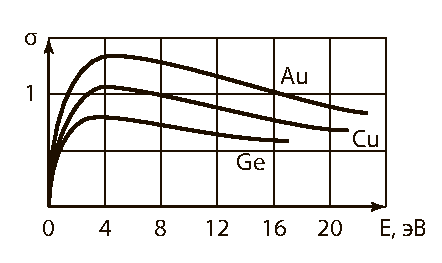
\includegraphics[width=.47\textwidth]{05_1}
    \caption{Кривые зависимости коэффициента вторичной эмиссии от энергии 
        первичных электронов}
    \label{img05.1}
\end{figure}

Отметим, это типичная кривая \( \sigma(Е_p) \) представляет собой кривую с 
экстремумом в области \( E_p = E_{pm} \). Используя этот факт, в качестве 
простейшего варианта оценки можно использовать соотношение
\begin{equation}
    \frac{\sigma}{\sigma_m} = 4\left( \frac{E_p}{E_{pm}} \right)
        \left( 1 + \frac{E_p}{E_{pm}} \right)^{-2}
    \label{eq05.1.19}
\end{equation}
полученное Кадышевичем. В (\ref{eq05.1.19}) \( \sigma_{m} \) -- максимальное 
значение коэффициента вторичной эмиссии, \( E_p \) -- энергия падающего 
первичного электрона, \( Е_{pm} \) -- энергия, при которой достигается 
экстремум кривой. Уменьшение \( \sigma \) с ростом \( E_p > E_{pm} \) 
обусловлено тем фактом, что первичные электроны глубоко проникают в материал 
эмиттера и возбуждают электроны, находящиеся в его глубине. Несмотря на 
возбуждение, вероятность выхода таких электронов из мишени очень мала.

Другой важной характеристикой вторичной эмиссии является распределение 
испускаемых электронов по энергиям. Поскольку вторичные электроны вылетают 
из эмиттера по разным направлениям и с разными энергиями при фиксированных 
величинах энергии падающих электронов \( E_p \), то для точечного источника 
вторичных электронов полный коэффициент вторичной эмиссии может быть определен 
из соотношения
\begin{equation}
    \sigma = \int\limits_{0}^{E_p} dE \int\limits_{0}^{2\pi} d\phi 
        \int\limits_{0}^{\pi/2} f(E,\bar{\Sigma})\sin\theta d\theta
    \label{eq05.1.20}
\end{equation}

Здесь \( \bar{\Sigma}(\phi,\theta) = \vec{v}/v \) -- единичный вектор, 
задающий направление скорости вторичного электрона, \( Е \) -- его энергия, 
ось \( z \)  направлена по нормали к поверхности эмиттера (используется 
сферическая система координат), \( f(E,\bar{\Sigma} \) -- функция 
распределения электронов вторичных электронов по энергиям и направлениям 
вылета, \( \sin\theta d\phi d\theta \) -- элемент телесного угла. Соотношение 
(\ref{eq05.1.20}) записано для эмиссии на отражение, то есть когда вторичный 
поток электронов эмитируется в то же пространство, откуда прилетают первичные 
электроны.

Энергетический спектр электронов определяется выражением
\begin{equation}
    F(E) = \int\limits_{0}^{2\pi} d\phi 
        \int\limits_{0}^{\pi/2} f(E,\bar{\Sigma}) \sin\theta d\theta
    \label{eq05.1.21}
\end{equation}

Несмотря на различие материалов, которые могут выполнить роль эмиттера 
вторичных электронов, кривые распределения \( F(E) \) имеют общие черты, 
характерные для всех веществ. На рис.\ref{img05.2} представлена типичная 
зависимость \( F(E) \) для меди, на которой просматриваются два четких 
максимума: один из них соответствует \( Е = E_p \) и определяет группу упруго 
отраженных от мишени первичных электронов, второй лежит в интервале энергий от 
1 до 4–6 эВ. Он определяет наиболее вероятную энергию в группе медленных 
электронов. Интересно отметить, что положение максимума в низковольтной 
области спектра  для  данного  материала практически не меняется при изменении 
\( E_p \) в широких пределах.

Величина вторичной эмиссии зависит также и от угла падения первичных 
электронов на мишень. Действительно, первичные электроны, двигаясь внутри 
вещества прямолинейно, при наклонном падении проникают вглубь тела на меньшую 
глубину, чем при нормальном падении. При одинаковых возможностях возбуждения 
вторичных электронов, вероятность выхода при наклонном падении первичного 
пучка выше. Это явление характерно для всех материалов эмиттера, но угловая 
зависимость величины \( \sigma \) в этом случае проявляется более резко для 
легких и менее резко -- для тяжелых элементов. Если же поверхность 
шероховатая, то \( \sigma \) практически от угла не зависит.
\begin{figure}[h]
    \center
    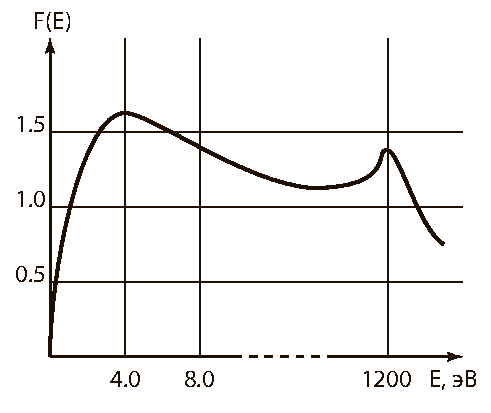
\includegraphics[width=.47\textwidth]{05_2}
    \caption{Распределение вторичных электронов по энергиям для меди 
        \( E_p = 1200 \) эВ}
    \label{img05.2}
\end{figure}

Вторичные эмиссии электронов наблюдаются и тогда, когда на поверхность 
вещества падает поток ионов. Это явление может играть как положительную, так 
и отрицательную роль, поэтому его всегда надо учитывать на практике.
